\cotefile{162-5}

\scanpage{47}
catégorie \inserted{additive(et même quasi-abélienne)}avec $\otimes$ qui a toutes les vertus,sauf d'être abélienne, et
sauf d'admettre des \uline{Hom} internes. Pour trouver ces derniers, on peut
si on veut paraphraser la construction de la catégorie des motifs, en
\deleted{introduisant un motif} considérant l'objet \inserted{$\handwritten{\Lambda}(-1)$} de $\tilde{\underline{B}}$ conoyau de
$p^{\handwritten{\unsure{*|\alpha}}}$ : $e \handwritten{\longrightarrow} S$, où $p:S^{1} \handwritten{\longrightarrow} e$ est l'application du cercle sur un
point. C'est un objet de poids 1 (le poids est défini par le degré \deleted{d}
des générateurs, changés de signe). On constate aussitôt que le
foncteur $M\handwritten{\mapsto} M(-1)=M\otimes\handwritten{\Lambda}(-1)$ de $\tilde{\underline{B}}$ dans lui-même est pleinement fidèle,
ce qui permet alors, par une construction formelle standard, de complé%
ter $\tilde{\underline{B}}$ en une catégorie où $\handwritten{\Lambda}(-1)$ devient inversible. Il se trouve
alors que dans cette dernière les \uline{Hom}(X,Y) internes existent et
\deleted{satisfont} sont isomorphes à $\check{X}\otimes Y$ ... en fait , on trouve maintenant la
catégorie de\deleted{s} \uline{tous} les modules gradués libres de type fini sur \quad .
Bien sûr, cette catégorie n'est pas encore abélienne pour autant,
puisque \quad n'est pas un corps; \deleted{pour} \inserted{si on veut} définir la catégorie abélienne
engendrée, on s'attend à trouver l\deleted{\unsure{e}}a\deleted{s} catégorie \handwritten{/}des\handwritten{/}modules de \deleted{type} \inserted{\handwritten{présentation}} fini\inserted{\handwritten{e}}
sur $\handwritten{\Lambda}$.( \inserted{\handwritten{qui est abélienne bien que $\Lambda$ ne soit pas noethérien, car $\Lambda$ est}} \deleted{\quad est-il noethérien, j.e. le nombre de générateurs est-il}
\margin{\handwritten{\unsure{Non|?}}}\deleted{fini ? )\unsure{.}} \handwritten{$\varinjlim$ d'anneaux noeth\unsure{.|,} à hom\unsure{s} de transition \uline{plats}).}

Cette construction ressemblerait à celle d'une théorie des
motifs où on n'aurait pas passé à l'équivalence homologique pour
les cycles, mais où on aurait gardé l'équivalence rationelle, - qui
est bien trop fine \deleted{pou\unsure{r}}à beaucoup d'égards. Pour trouver un équiva\deleted{l}%
lent plus étroit, il convi\deleted{n}e\deleted{t}nt de reprendre la théorie pré\unsure{\deleted{d}c|d}édente,on
pourrait formuler le même Pb universel que plus haut, mais en prenant
l'équivalence homologique (via le graphe) des morphismes de variétés,
au lieu de l'équivalence homotopique. \deleted{Mais alors il semble que l'on
trouve comme catégorie solution celle dont les objets sont les varié-}

\margin{\handwritten{46}}

\scanpage{48}
\deleted{tés, les morphismes \uline{toutes} les correspondances \inserted{co}homologiques (en vert\unsure{u}
du thorème de Thom rappelé plus haut). On trouve donc un foncteur
pleineme\deleted{t}nt fidèle de cette catégorie dans celle d es vectoriels
gradués \deleted{\unsure{de d}} positivement de dim. finie sur $\underline{F}_2$ , qui est déjà abélien%
ne, et si on veut rendre comme plus haut $\underline{F}_2(-1)$ inversible, on trouve
tous les vectoriels gradués de dim. finie sur $\underline{F}_2$ . C'est un peu trop
trivial comme structure, et on peut faire mieux, \deleted{en prenant comme}}

\inserted{Pour trouver une catégorie universelle,}
\deleted{\unsure{correspondances. Pour ceci}} on associe à toute X \deleted{\unsure{le sous-anneauensemble}}
\deleted{\unsure{de}} l'ensemble \inserted{S(X)} des sous-variétés \deleted{S(X)} de X, modulo équivalence homolo%
gique. Donc S(X) \handwritten{$\subset$} $H^{\cdot}(X)$, et on prouve qu'on trouve en fait un sous-
anneau de $H^{\cdot}(X)$ (grâce à un théorème de Thom qui caractérise S(X) en
termes d'opérations de Steenrod, cf plus bas). On prouve de même
(par le même théorème) que les S(XxY) sont stables par composition des
correspondances cohomologiques\deleted{\illegible{1}}( cela ne semble pas trivial, puisque
les S(X) ne sont pas stables par Gysin...). D'o\unsure{û|ù} une catégorie addi-
tive dont les objets sont ceux de C, les flêches sont les S(XxY),
Il semble qu'elle doive jouer le rôle universel que j'ai envisagé
plus haut. En tous cas, sa définition géo\deleted{é}m\deleted{m}étrique est fort simple !
Nous allons en donner une interpétation algébrique. P\u{o}ur ce\deleted{i}c\deleted{c}i,
considérons l'anneau des opérations cohomologiques \inserted{``stables''} \deleted{\deleted{additives sur} i.e.}
\margin{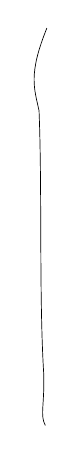
\begin{tikzpicture}[x=0.01cm,y=0.01cm]\draw[line width=.25pt] (17,505) .. controls (-7,446) and (1,428) .. (7,400) .. controls (11,300) and (7,160) .. (13,65) .. controls (14,25) and (8,13) .. (15,0);\end{tikzpicture}}
\deleted{\inserted{des endomorphismes du}}
\margin{\handwritten{\unsure{Faux !|?}}}
\deleted{\deleted{le} foncteur X \quad $H^{\cdot}$(X) qui sont additifs, et qui en degré zéro se
réduisent à un multiple de l'identité.} C'est un anneau gradué, avec
application diagonale anticommutative, \inserted{i.e. commutative (car. 2 !)} associative et unitaire. Son
dual gradué est une algèbre \inserted{graduée an\unsure{ti|tt}commutative donc \deleted{commutative},} commutative,avec application diagonale
associative et unitaire; il est réduit à $\underline{F}_2$ en degré zéro. Donc il
corespond à un schéma en groupes \handwritten{aff}ine G sur $\underline{F}_2$ , qui est d'ailleurs
le foncteur des $\otimes$-automorphismes \inserted{additifs} du foncteur $H^{\cdot}$ sur C \inserted{\handwritten{qui opèrent
trivialement sur \deleted{\unsure{l'objet}} $H^{\unsure{1}}(S^1)$. \deleted{\illegible{1}}}}

\margin{\handwritten{47}}

\scanpage{49}
Le théorème de Thom est alors qu'un $x \handwritten{\in} H^{\cdot}(X)$ est dans S(X) sss il est
\deleted{stable}\inserted{fixe} par G, i.e. satisfait $A^{\handwritten{+}}. x = 0$. (Pourquoi cette condition est-el\deleted{\unsure{l}}%
le déjà nécessaire ?) U\handwritten{n}e autre façon de le voir est de dire que le
foncteur $H^{\cdot}$ considéré comme allant de la catégorie $\underline{S}$ précédente dans
la catégorie des \deleted{vectoriels} représentations de G dans des vectoriels
sur $\underline{F}_2$ , est pleinement fidèle. \deleted{Comme G \unsure{n'|est|et}} Quand on prend l'enveloppe
pseudo-abélienne, on trouve une sous-catégorie pleine de la catégorie des
représentations de G, mais il est douteux qu'on trouve une catégorie abé-%
lienne, voire la catégorie de toutes les représentations de G de dimensio
finie sur $\underline{F}_2$ . (Quelle est la structure de G, qui est prolisse; d'après
\margin{\handwritten{oui, car son anneau affine est une algèbre de polynômes à une infinité d'indéterminées, \deleted{\illegible{1}} réunion d'algèbres de polynômes à \unsure{engendrement} fini \unsure{stables} par $\Delta$}}Quillen, il serait pro-unipotent ....). Ici G bien sûr joue le rôle d'un
groupe de Galois motivique, mais contrairement à la situation familière,
il semble qu'il soit fortement non réductif (et d'ailleurs le corps de
définition dans tout ceci est $\underline{F}_2$ , et non $\underline{Q}$ ! ).

Quillent donne une généralisation de la construction d'une caté-%
gorie universelle $\underline{B}$ au cas où on travaille avec des variétés pas né\unsure{c|e}essai%
rement propres (mais f. n'étant supposé défini que pour f propre), et
quand on introduit une condition d'orientation \inserted{stable} sur les \uline{morphismes}
envisagés , via un morphisme $H \handwritten{\to BO(\infty)}$, où H est un H-espace (commuta%
tif, associatif et unitaire ?): une orientation de $f:X \handwritten{\to} Y$ sera un
relèvement homotopique de $X \handwritten{\to BO}$ défini par \deleted{$f^{\cdot}(T$} $T_X - f^{\cdot}(T_Y)$ en $X \handwritten{\to} H$.
les éléments de H(X,Y) seront définis par des diagrammes de morphismes
orientés $Z \handwritten{\to} X$, $Z \handwritten{\leftarrow} Y$, le deuxième étant propre, modulo bords de tels.
En tant qu'ensemble, il se définit aussi en termes de la vari té $X\mathrm{x}Y$
munie simplement de la famille des supports formée des ensembles fermés
propres sur Y ..... \handwritten{Les $B^{H}_{m}(X)$ (X compact disons) peuvent}
\handwritten{se dé\unsure{crire|finir} homotopiquement à la Thom, comme les groupes d'homotopie}
\handwritten{stables d'espaces $\underline{\mathrm{Hom}}(X, MH(N-m))$ - - - - -.}

\margin{\handwritten{48}}

\scanpage{51}
Inventiones math. 5, 237--242 (1968)

On the Representation of Hermitian Forms
as Sums of Squares

\textsc{Daniel G. Quillen}\textsuperscript{*} (Cambridge, Mass.)

There is an extensive literature (e.g. [1], Ch.VI) concerned with
Hilbert's problem of representing a positive-valued form with real
coefficients as a sum of squares. The corresponding problem for her-%
mitian forms does not seem to have been touched. In this paper we
present a theorem about hermitian forms which arose in connection
with a priori estimates for partial differential equations. This theorem is
proved by the methods of a priori estimates and one of its corollaries
is the Hilbert Nullstellensatz over $\mathbf{C}$, so we obtain a direct analytic proof
of the latter theorem.

Let $T$ and $V$ be finite dimensional complex vector spaces and let
$E(u_1,u_2)$ be a hermitian form on $S_m T\otimes V$ where $S_m$ denotes $m$-th sym-%
metric tensors. If $\zeta\in T$ and $v\in V$ let
\[ E^{\wedge}(\zeta,v)=(m!)^{-2}\,E(\zeta^m\otimes v,\zeta^m\otimes v). \]
Then $E^{\wedge}$ is a real-valued smooth function on $T\times V$ such that
\[ E^{\wedge}(s\,\zeta,t\,v)=|s|^{2m}\,|t|^2\,E^{\wedge}(\zeta,v) \tag{1} \]
for $s,t\in\mathbf{C}$, and the map $E\mapsto E^{\wedge}$ yields a 1-1 correspondence between
hermitian forms on $S_m T\otimes V$ and smooth functions on $T\times V$ satisfying (1).
The inverse procedure of passing from a function to a form is polariza-%
tion (see formulas (2) below).

Let $|\zeta|^2$ be a hermitian scalar product on $T$ and define the ``$N$-th
prolongation'' of $E$ to be the hermitian form $E^N$ on $S_{m+N}T\otimes V$ with
\[ (E^N)^{\wedge}(\zeta,v)=(N!)^{-1}\,|\zeta|^{2N}\,E^{\wedge}(\zeta,v). \]
\textbf{Theorem.} \emph{The following conditions are equivalent:}

(i) \emph{$E^{\wedge}(\zeta,v)>0$ for $\zeta\neq 0$ and $v\neq 0$.}

(ii) \emph{For sufficiently large $N$, $E^N$ is positive definite.}

We first derive an expression for $E^N$ as an integral. By choosing an
orthonormal basis for $T$ we may identify $T$ with the space of $\mathbf{C}$-linear
functions on $\mathbf{C}^n$ in such a way that the orthonormal basis is $z^1,\dots,z^n$
where $z^i$ is the $i$-th coordinate function. Then $S_k T$ may be naturally
identified with the holomorphic polynomial functions homogeneous of

* This research was supported in part by NSF GP-6959.

17 Inventiones math., Vol. 5

\margin{\handwritten{50}}

\scanpage{52}
\mspage{238} \hfill D.G. Quillen:

degree $k$ and $S_k T$ has the basis $z^\alpha$, $|\alpha|=k$ where $\alpha$ is a multi-index. If we
identify $V$ with $\mathbf{C}^r$ and let $e_1,\dots,e_r$ be the canonical basis of $\mathbf{C}^r$, then
$S_k T\otimes V$ can be naturally identified with the holomorphic polynomial
functions homogeneous of degree $k$ with values in $\mathbf{C}^r$. Then $S_m T\otimes V$
has the basis $z^\alpha e_i$, $|\alpha|=m$, $1\leqq i\leqq r$, so there are complex numbers $a_{\alpha i,\beta j}$,
$|\alpha|=|\beta|=m$, $1\leqq i, j\leqq r$ with $a_{\beta j,\alpha i}=a^*_{\alpha i,\beta j}$ such that
\[
\begin{aligned}
E(u_1,u_2)&=\sum \alpha!\,\beta!\,a_{\alpha i,\beta j}\,b_{\alpha i}\,c^*_{\beta j}\\
E^\wedge(\zeta,v)&=\sum a_{\alpha i,\beta j}\,\zeta^\alpha\,v_i\,\zeta^{*\beta}\,v^*_j
\end{aligned}
\tag{2}
\]
if $u_1=\sum b_{\alpha i}\,z^\alpha e_i$, $u_2=\sum c_{\alpha i}\,z^\alpha e_i$, $\zeta=\sum \zeta^i z^i$, and $v=(v_1,\dots,v_r)$, where *
denotes complex conjugate. The matrix $a_{\alpha i,\beta j}$ may be determined from
the Taylor series of $E^\wedge$ at $(0,0)$ which shows that $E$ and $E^\wedge$ determine
each other.

Let $E^\sim$ be the differential quadratic form
\[
E^\sim(f,g)=\sum a_{\alpha i,\beta j}(D^\alpha f_i)(D^\beta g_j)^*
\]
where $f$ and $g$ are holomorphic functions on $\mathbf{C}^n$ with values in $\mathbf{C}^r$ and
$D^i=\partial/\partial z^i$. If $dG=\pi^{-n}\exp(-|z|^2)\,dx^1\,dy^1\dots dx^n\,dy^n$ is the Gaussian
measure on $\mathbf{C}^n$, then we have the following expression for $E^N$.

\textbf{Lemma 1.} \textit{If $f,g\in S_{m+N}T\otimes V$, then}
\[
E^N(f,g)=\int E^\sim(f,g)\,dG.
\]

\textit{Proof.} If $u_1$, $u_2$ are two holomorphic polynomial functions on $\mathbf{C}^n$, let
\[
(u_1,u_2)_0=\int u_1\,u_2^*\,dG.
\]

By integrating by parts we obtain the basic formula
\[
(D^i u_1,u_2)_0=(u_1,z^i u_2)_0,
\]
from which follows
\[
(z^\alpha,z^\beta)_0=\begin{cases}0 & \alpha\neq\beta\\ \alpha! & \alpha=\beta.\end{cases}
\tag{3}
\]
By definition
\[
\begin{aligned}
(E^N)^\wedge(\zeta,v)&=(N!)^{-1}\,|\zeta|^{2N}\,E(\zeta,v)=\sum_{|\gamma|=N}(\gamma!)^{-1}\,\zeta^\gamma\,\zeta^{*\gamma}\,E(\zeta,v)\\
&=\sum(\gamma!)^{-1}\,a_{\alpha i,\beta j}\,\zeta^{\gamma+\alpha}\,v_i(\zeta^*)^{\gamma+\beta}\,v_j^*,
\end{aligned}
\]
hence
\[
(E^N)^\sim(f,g)=\sum_{|\gamma|=N}(\gamma!)^{-1}\,E^\sim(D^\gamma f,D^\gamma g).
\]
By linearity it suffices to prove the lemma when $f=z^\delta e_i$ and $g=z^\varepsilon e_j$
where $|\delta|=|\varepsilon|=m+N$. But
\[
E^N(f,g)=(E^N)^\sim(f,g)(0)=\sum_{\substack{|\alpha|=|\beta|=m\\ |\gamma|=N}}(\gamma!)^{-1}\,a_{\alpha i,\beta j}(D^{\gamma+\alpha}z^\delta)(D^{\gamma+\beta}z^\varepsilon)^*
\]

\margin{\handwritten{51}}

\scanpage{53}
On the Representation of Hermitian Forms as Sums of Squares \mspage{239}

and
\[ \int E^{\sim}(f,g)\,dG = \sum_{|\sigma|=|\tau|=m} a_{\sigma i,\tau j}(D^{\sigma} z^{\delta}, D^{\tau} z^{\varepsilon})_0 . \]
These two coincide by (3), proving the lemma.

Introduce norms
\[ \|u\|_q^2 = \int \sum_{|\gamma|=q} (\gamma!)^{-1}\, |D^{\gamma} u|^2\, dG \]
\[ \|u\|_{q*}^2 = \int (q!)^{-1}\, |z|^{2q}\, |u|^2\, dG \]
where $u \in S_* T \otimes V$ is thought of as a function with values in $V$ and $|v|^2 =$
$\sum v_i v_i^*$. Let $(\ ,\ )_q$ and $(\ ,\ )_{q*}$ be the associated hermitian forms. Let
$C_k{}^q$ be the binomial coefficients.

\textbf{Lemma 2.} \emph{If $u \in S_k T \otimes V$, then $\|u\|_q^2 = C_q{}^k\, \|u\|_0^2$.}

\emph{Proof.} By the binomial theorem
\[ \sum_{\gamma} C_{\gamma}{}^{\delta} X^{\gamma} = (1+X)^{\delta} \]
where $C_{\gamma}{}^{\delta} = \delta!\,(\gamma!\,(\delta-\gamma)!)^{-1}$ and $X=(X_1,\dots,X_n)$. Substituting $X_1 = \cdots =$
$X_n = t$ and comparing coefficients of $t^q$ we have
\[ \sum_{|\gamma|=q} C_{\gamma}{}^{\delta} = C_q{}^{|\delta|}. \tag{4} \]
Using (3) and (4) we have
\[ \begin{aligned} \|z^{\alpha} e_i\|_q^2 &= \sum_{|\gamma|=q} (\gamma!)^{-1}\, \|D^{\gamma} z^{\alpha}\|_0^2 = \sum_{|\gamma|=q} (\gamma!)^{-1}\, (\alpha!)^2\, ((\alpha-\gamma)!)^{-1} \\
&= \alpha!\, C_q{}^{|\alpha|} = C_q{}^k\, \|z^{\alpha} e_i\|_0^2 . \end{aligned} \]
Combining this with the readily verified fact that $z^{\alpha} e_i$ and $z^{\beta} e_j$ in $S_k T \otimes V$
are orthogonal for both $(\ ,\ )_q$ and $(\ ,\ )_0$ unless $\alpha=\beta$ and $i=j$, we obtain
the lemma.

\textbf{Lemma 3.} \emph{There is a constant $C$ depending only on $q$ such that}
\[ \|u\|_q^2 \leqq \|u\|_{q*}^2 \leqq C \sum_{j \leqq q} \|u\|_j^2 \]
\emph{for every $u$ in $S_* T \otimes V$.}

\emph{Proof.} We shall need the commutation formulae
\[ \begin{aligned} (\alpha!\,\beta!)^{-1} z^{\alpha} D^{\beta} u &= \sum_{\gamma} (-1)^{|\gamma|}\, (\gamma!\,(\beta-\gamma)!\,(\alpha-\gamma)!)^{-1}\, D^{\beta-\gamma} z^{\alpha-\gamma} u \\
(\alpha!\,\beta!)^{-1} D^{\alpha} z^{\beta} u &= \sum_{\gamma} (\gamma!\,(\beta-\gamma)!\,(\alpha-\gamma)!)^{-1}\, z^{\beta-\gamma} D^{\alpha-\gamma} u \end{aligned} \tag{5} \]
where the first may be obtained as the coefficient of $s^{\alpha} t^{\beta}$ in the power
series expansion of the Weyl commutation relations
\[ e^{sz} e^{tD} u(z) = e^{-st} e^{tD} e^{sz} u(z) \]
\[ \text{i.e. } e^{sz} u(z+t) = e^{-st} e^{s(z+t)} u(z+t) \]

17*

\margin{\handwritten{52}}

\scanpage{54}
\mspage{240} D. G. Quillen:

and where the second may be derived similarly (see also [2], p. 153). Thus
\[ \|u\|^2_{q*} = \sum_{|\alpha|=q} (\alpha!)^{-1}\, \|z^\alpha u\|^2_0 = \sum_{|\alpha|=q} (\alpha!)^{-1} (u, D^\alpha z^\alpha u)_0 \]
\[ = \sum_{|\alpha|=q} \sum_{\gamma} \alpha!\,(\gamma!\,(\alpha-\gamma)!^2)^{-1} (u, z^{\alpha-\gamma} D^{\alpha-\gamma} u)_0 \]
\[ = \sum_{|\alpha|=q} \sum_{\gamma} C_\gamma{}^\alpha ((\alpha-\gamma)!)^{-1}\, \|D^{\alpha-\gamma} u\|^2_0 \]
from which the lemma immediately follows.

\emph{Proof of the Theorem.} The implication (ii)$\Rightarrow$(i) is clear, so assume (i)
holds. If $u \in S_{m+N}\, T \otimes V$ then by Lemma 1, (2), and (5) we have with
indices running like $1 \leqq i,\ j \leqq r$, $|\alpha| = |\beta| = m$
\[ E^N(u,u) = \sum a_{\alpha i, \beta j} (D^\alpha u_i, D^\beta u_j)_0 \]
\[ = \sum a_{\alpha i, \beta j} (u_i, z^\alpha D^\beta u_j)_0 \]
\[ = \int \sum (-1)^{|\gamma|}\, a_{\alpha i, \beta j}\, \alpha!\, \beta!\, (\gamma!\, (\beta-\gamma)!\, (\alpha-\gamma)!)^{-1}\, z^{\beta-\gamma} u_i (z^{\alpha-\gamma} u_j)^*\, dG \]
\[ = \int [E^\wedge (z^*, u) + Q(z,u)]\, dG \]
where $Q(z,u)$ is of degree $<m$ in $z_i z_j^*$ and of degree 1 in $u_i u_j^*$. Thus
for some constant $C$
\[ |Q(z,u)| \leqq C \sum_{i<m} (i!)^{-1}\, |z|^{2i}\, |u|^2, \]
while by hypothesis on $E$ there is an $\varepsilon > 0$ such that
\[ |E^\wedge (z^*, u)| \geqq \varepsilon (m!)^{-1}\, |z|^{2m}\, |u|^2. \]
Therefore
\[ E^N(u,u) \geqq \int (\varepsilon (m!)^{-1}\, |z|^{2m} - C \sum_{i<m} (i!)^{-1}\, |z|^{2i})\, |u|^2\, dG \]
\[ = \varepsilon\, \|u\|^2_{m*} - C \sum_{i<m} \|u\|^2_{i*} \]
\[ \geqq \varepsilon\, \|u\|^2_m - C' \sum_{i<m} \|u\|^2_i \]
using Lemma 3. By Lemma 2 we have $E^N(u,u) \geqq P(N)\, \|u\|^2_0$ where
\[ P(N) = \varepsilon\, C_m{}^{m+N} - C' \sum_{i<m} C_i{}^{i+N} \]
is a polynomial of degree $m$ in $N$ with positive leading coefficient. Thus
for $N$ sufficiently large $P(N) > 0$ so $E^N$ is positive definite and the theorem
is proved.

We shall now give some applications of the theorem when $V = \mathbf{C}$
and $T = \mathbf{C}^n$.

\margin{\handwritten{53}}

\scanpage{55}
On the Representation of Hermitian Forms as Sums of Squares \mspage{241}

\textbf{Corollary 1.} \emph{Let}
\[ E^{\wedge}(\zeta)=\sum_{|\alpha|=|\beta|=m} a_{\alpha\beta}\,\zeta^{\alpha}\,\zeta^{*\beta} \]
\emph{be a hermitian form homogeneous of degree $m$ on $\mathbf{C}^n$ which is strictly
positive, i.e. $E^{\wedge}(\zeta)>0$ if $\zeta\neq 0$. Then for sufficiently large $N$,}
\[ E^{\wedge}(\zeta)=\frac{\sum\limits_{i}|P_i(\zeta)|^2}{\sum\limits_{|\gamma|=N}(\gamma!)^{-1}\,|\zeta^{\gamma}|^2} \]
\emph{where $P_i(\zeta)$ is a basis for the holomorphic polynomials of degree $m+N$ on $\mathbf{C}^n$.}

\textbf{Corollary 2.} \emph{Let}
\[ E^{\sim}(f)=\sum_{|\alpha|=|\beta|=m} a_{\alpha\beta}\,D^{\alpha}f(D^{\beta}f)^* \]
\emph{be a differential quadratic form in $n$ variables homogeneous of degree
$(m,m)$, such that $a_{\beta\alpha}=a^*_{\alpha\beta}$. If $E^{\sim}$ has no non-zero characteristics, i.e.
$\sum a_{\alpha\beta}\,\zeta^{\alpha}\,\zeta^{*\beta}>0$ for $\zeta\neq 0$, then for sufficiently large $N$ we may write}
\[ \sum_{|\gamma|=N}(\gamma!)^{-1}\,E^{\sim}(D^{\gamma}f)=\sum_{i}|P_i(D)\,f|^2 \]
\emph{where $P_i(D)$ is a basis for the homogeneous polynomials of degree $m+N$
in $D_1,\dots,D_n$.}

These corollaries are just reinterpretations of the implication (i)$\Rightarrow$(ii)
of the theorem.

\emph{Example.} Let $E^{\sim}(f)=|D_1^2\,u|^2-|D_1\,D_2\,u|^2+|D_2^2\,u|^2$ where $n=2$. The dif-%
ferential quadratic form $E^{\sim}$ is not a sum of squares because $E^{\sim}(z^1\,z^2)<0$.
But $E^{\sim}(\zeta)=(|\zeta_1|^2-|\zeta_2|^2)^2+|\zeta_1\,\zeta_2|^2>0$ if $\zeta\neq 0$ so the theorem applies.
In fact $E^{1\sim}(f)=|D_1^3\,f|^2+|D_2^3\,f|^2$ and $E^N$ is positive definite for $N\geqq 3$.

\textbf{Corollary 3.} \emph{(Projective Nullstellensatz over $\mathbf{C}$.) If $Q_j(z)$ $1\leqq j\leqq l$ are
homogeneous polynomials in $z^1,\dots,z^n$ without a common zero $\zeta\neq 0$, then
the ideal generated by the $Q_j$ contains all homogeneous polynomials of
sufficiently high degree.}

\emph{Proof.} We may assume that the $Q_j$ have the same degree $m$. Let
\[ E^{\wedge}(\zeta)=\sum_{j}|Q_j(\zeta)|^2; \]
then $E^{\wedge}(\zeta)>0$ if $\zeta\neq 0$ so by Corollary 2 for all sufficiently high $N$, there
is an expression
\[ \sum_{j}\sum_{|\gamma|=N}(\gamma!)^{-1}\,|D^{\gamma}\,Q_j(D)\,f|^2=\sum|P_i(D)\,f|^2 \]
where $P_i(D)$ is a basis for the space $W$ of homogeneous polynomials
of degree $m+N$. It follows that the set $D^{\gamma}\,Q_j(D)$ for $|\gamma|=N$, $1\leqq j\leqq l$
spans $W$ for otherwise we could take $f$ to be a non-zero polynomial in

\margin{\handwritten{54}}

\scanpage{56}
\mspage{242} D.G. Quillen: On the Representation of Hermitian Forms as Sums of Squares

$z$ homogeneous of degree $m+N$ killed by the $D^\gamma Q_j(D)$ and get a contra-%
diction. This proves the corollary.

Corollary 3 implies the usual Nullstellensatz by means of the Rabino-%
witz trick and making polynomials homogeneous by adding an extra
variable. Hence we have given a direct analytical proof of the Null-%
stellensatz over $\mathbf{C}$ bearing some resemblance to the Liouville theorem
proof of the fundamental theorem of algebra.

\begin{center}
\textbf{Bibliography}
\end{center}

1. Jacobson, N.: Lectures in abstract algebra III. Princeton: van Nostrand 1964.

2. Trèves, F.: Linear partial differential equations with constant coefficients. New York:
Gordon \& Breach 1966.

\begin{flushright}
\begin{tabular}{l}
Dr. D. G. Quillen\\
Massachusetts Institute of Technology\\
Department of Mathematics\\
Cambridge, Mass. 02139, USA
\end{tabular}
\end{flushright}

\begin{center}
\textit{(Received February 27, 1968)}
\end{center}

\margin{\handwritten{55}}

\scanpage{58}

\begin{center}
\uline{On a conjecture of Adams}*

\handwritten{D.G. Quillen}
\end{center}

This conjecture asserts that if $X$ is a finite CW complex
and $x \in K(X)$ , then for $n$ sufficiently large $p^{n}(\handwritten{\psi}^{p}x - x)$ repre-%
sents $0$ in $J(X)$ . Here $p$ is a prime number and $K$ is complex
$K$ theory. (Actually Adams states the conjecture when $p$ is any
integer and for real $K$ theory. It is clearly sufficient to prove
the result when \handwritten{$p$} is prime. We shall restrict ourselves entirely
to complex vector bundles for our methods do not apply to real $K$
theory.) Adams \handwritten{[1]} proves this conjecture if $x$ is a virtual sum
of line bundles \handwritten{and} reduces the conjecture for some other spaces
such as spheres \handwritten{to} this case. In this note we show how the etale
homotopy theory recently developed by Artin and Masur [2], which
extends the etale cohomology theory of Artin and Grothendieck [3],
may in principle be used to give a proof of this conjecture. Actu-%
ally there are certain results for the etale homotopy theory which
we need and which at the moment have not been proved, so this note
is really a sketch of a potential proof of this conjecture. How-%
ever the possibility of proving a theorem about CW complexes
using algebraic varieties in characteristic $p$ seems sufficiently
startling to merit publication in this incomplete form.

We begin by describing our key idea. In [1] Adams shows that
two vector bundles \handwritten{$E$} and \handwritten{$F$} over $X$ represent the same element
of $J(X)$ mod $p$-torsion if there exists a fiber preserving map

\noindent\rule{0.4\textwidth}{0.4pt}

*This research \handwritten{was} supported \deleted{\unsure{in part}} by \deleted{\unsure{a grant from the}}
\deleted{\unsure{National Science Foundation}} \inserted{\handwritten{\unsure{NSF GP 6106|NSF GP 6109|NSF GP 6100|NSF GP 6166}}}.

\margin{\handwritten{57}}

\scanpage{59}
$f:E - 0 \rightarrow F - 0$ which is of degree a power of $p$ on each fiber.
When $E$ is a line bundle, then $\handwritten{\psi}^pE = E^{\otimes p}$ and $f(v) = v^{\otimes p}$ is
the desired map to prove the conjecture for $E$ . Unfortunately
when $E$ has dimension greater than one, then $\handwritten{\psi}^pE$ is only a vir-%
tual bundle so the method fails. However if $E$ is an algebraic
vector bundle (locally free sheaf of finite rank) over a prescheme
$V$ of characteristic $p$ , then in virtue of the Frobenius homomor-%
phism there is an algebraic vector bundle $E^{(p)}$ whose class in
$K_{alg}(V)$ represents $\handwritten{\psi}^pE$ .\textsuperscript{\handwritten{*}} If $E$ is given by a cocycle $(g_{ij})$ of
$n\mathrm{x}n$ matrices with respect to an open covering of $V$ , then $E^{(p)}$
is given by the cocycle $(g_{ij}^{(p)})$ , where $g_{ij}^{(p)}$ denotes the matrix
whose entries are the p-th powers of the corresponding entries of
$g_{ij}$ . Moreover there is a canonical map $F:E \rightarrow E^{(p)}$ given in lo-%
cal coordinates by $(X_i) \rightarrow (X_i^p)$ which is of (inseparable) degree
$p^{\handwritten{\dim E}}$ on each fiber. Hence the hypotheses for Adams' criterion is
verified in the algebraic situation and it remains to reduce the
topological situation to the algebraic one.

It evidently suffices to prove the conjecture when $X$ is the
Grassmannian of complex $N$ planes in $n + N$ space and where
$x \in K(X)$ is the class of the canonical quotient bundle. Let $G_Z$
be the Grassmannian scheme over Spec Z representing the functor
``isomorphism classes of n-dimensional vector bundles with $n + N$
generating sections'' and let $Q_Z$ be the canonical n-dimensional
bundle. Then $X = G_{C,cl}$ and $x$ is the class of $Q_{C,cl}$ , where

\handwritten{* That $E^{(p)}$ represents $\psi^pE$ follows since $E \mapsto E^{(p)}$ defines a
homomorphism $K_{alg} \rightarrow K_{alg}$ which coincides with $\psi^p$ on line bundles\unsure{;|,}
together with the splitting principle: $K_{alg}(PE) \cong K_{alg}(X)[T]/(\lambda_{-T}(E))$.}

\margin{\handwritten{58}}

\scanpage{60}
\mspage{- 3 -}

$G_A,Q_A$ denote the base extension of $G_Z,Q_Z$ by the map Spec A $\to$
Spec Z , and where if Y is a prescheme of finite type over Spec C,
$Y_{cl}$ denotes the set of complex points of Y with its ``classical''
topology. Let R be a strict localization of Z at the prime p
and choose an embedding R $\to$ C . Then R is a henselian discrete
valuation ring whose residue field k is algebraically closed of
characteristic p . Let $\underline{H}$ be the homotopy category of connected
pointed CW complexes, and let $X \to \hat{X}$ be the \uline{etale homotopy type}
functor [2] from the category of geometrically pointed locally con-%
nected preschemes to pro-$\underline{H}$. Let C be the class of finite groups
of order prime to p , and let $\underline{X} \to \hat{\underline{X}}$ be the \uline{C-completion} functor
[2] pro $\underline{H} \to$ pro C$\underline{H}$ \unsure{,|.} Choose a rational point of $G_Z$ over Spec Z
and rationally point $G_A$ by base extension. Then as $G_R$ is proper
and smooth over Spec R and 1-connected, the fundamental comparison
theorems of [2] imply that there are isomorphisms in pro-C$\underline{H}$

\diagram{
\begin{tabular}{@{}ll@{}}
(1)\qquad &
\begin{tikzcd}[column sep=large, ampersand replacement=\&]
G^{\wedge}_{C,cl} \arrow[r,"u"] \& G^{\wedge}_{C,et} \&
G^{\wedge}_{R,1,et} \arrow[l,"i"'] \arrow[r,phantom,"\overset{v}{\simeq}" description] \&
G^{\wedge}_{R,2,et} \& G^{\wedge}_{R,et} \arrow[l,"j"']
\end{tikzcd}
\end{tabular}
}

where i and j are base-change morphisms, u comes from the cano-%
nical map from the classical to the etale topology, where $G_{R,1}$
(resp. $G_{R,2}$) is the scheme $G_R$ with geometric point Spec C $\to$
Spec R $\to G_R$ (resp. Spec k $\to$ Spec R $\to G_R$) , and where v is the
isomorphism coming from shifting basepoints from 1 to 2 along the
``arc'' Spec R $\to G_R$ .

\margin{\handwritten{59}}

\scanpage{61}
\mspage{- 4 -}

We shall now \uline{assume} \deleted{for the moment} the possibility of defining
for each object $\underline{X}$ of pro-$C\underline H$ an abelian monoid $SF(\underline{X})$ of stable
isomorphism classes of oriented sphere fibrations with base $\underline{X}$ ,
such that there is a commutative diagram of monoids

(2)
\diagram{
\begin{tikzcd}[column sep=small, ampersand replacement=\&]
K(G_{C,cl}) \arrow[d, "J"] \& \& \&
K_{alg}(G_R) \arrow[lll, "aj^!"'] \arrow[rr, "i^!", "\handwritten{\sim}"'] \arrow[dl, "J"'] \arrow[dr, "J"] \& \&
K_{alg}(G_k) \arrow[d, "J"] \\
SF(G_{C,cl}) \arrow[r, "b"] \& SF(G^{\wedge}_{C,cl}) \&
SF(G^{\wedge}_{R,1,et}) \arrow[l, "u^*j^*"'] \arrow[rr, phantom, "\overset{v^*}{\simeq}" description] \& \&
SF(G^{\wedge}_{R,2,et}) \arrow[r, "i^*"] \& SF(G^{\wedge}_{k,et})
\end{tikzcd}
}

where $a:K_{alg}(G_C) \to K(G_{C,cl})$ is induced by the map associating to
an algebraic vector bundle $E$ the topological bundle $E_{cl}$ , where
$b$ is induced by sending $S^q \to W \to G_{C,cl}$ into $\widehat{(S^q)} \to \hat{W} \to G^{\wedge}_{C,cl}$ ,
and where $J$ is the map induced by sending an algebraic vector
bundle $E$ over $X$ into the sphere fibration $(E - 0)_{et} \to X_{et}$
which we denote by $\unsure{\$E|\phi E}$ .

With these assumptions we may now prove Adams' conjecture.
Denote by $cl(E)$ the class in $K$ or $K_{alg}$ of a vector bundle $E$ .
By the lemma at the end there is a vector bundle $E_R$ over $G_R$ with

\[ (3) \qquad cl(E_R) - n = \psi^p(clQ_R) - cl(Q_R) \]

Applying $i^!$ we obtain $cl(E_k) - n = \psi^p(clQ_k) - cl(Q_k) =$

\margin{\handwritten{60}}

\scanpage{62}
\mspage{- 5 -}

$\mathrm{cl}(Q_k^{(p)}) - \mathrm{cl}(Q_k)$ .  But  $F:Q_k - 0 \to Q_k^{(p)} - 0$  is fiber-preserving
and it is purely inseparable, hence a homeomorphism for the etale
topology.  Hence  $\$Q_k^{(p)} \simeq \$Q_k$  so  $i^*J(\mathrm{cl}E_R) = J(\mathrm{cl}(E_k) - n) = 0$ .
As  $i^*$ is an isomorphism by (1), $J(\mathrm{cl}E_R) = 0$, so from the diagram
(2) we find  $bJ\mathrm{cl}(E_{C,\mathrm{cl}}) = 0$ .  But this means that
\[ S^{2n-1} \to (E_{C,\mathrm{cl}} - 0)^{\wedge} \to G^{\wedge}_{C,\mathrm{cl}} \qquad , \]
is a stably trivial fibration, that is, there is a map  $u$  in
$\{(E_{C,\mathrm{cl}} - 0)^{\wedge} , S^{2n-1}\}$  such that  $u\hat{\epsilon} = \mathrm{id}$ .  Here  $\{ \; , \; \}$  denotes
S-maps in pro-$C\underline{H}$  [2] §8, and  $\epsilon:S^{2n-1} \to E_{C,\mathrm{cl}} - 0$  is the injection
of a fiber.  Consider the diagram

\diagram{
\begin{tikzcd}[column sep=small, ampersand replacement=\&]
\{(E_{C,\mathrm{cl}}-0) , S^{2n-1}\}^{\wedge} \arrow[r, "(\epsilon^*)^{\wedge}"] \arrow[d] \& \{S^{2n-1} , S^{2n-1}\}^{\wedge} \arrow[r, "v"] \handwritten{\arrow[d, line width=0.8pt]} \& Z/rZ \arrow[r] \arrow[d] \& 0 \\
\{(E_{C,\mathrm{cl}}-0)^{\wedge}, \widehat{S^{2n-1}}\} \arrow[r, "(\hat{\epsilon})^*"] \& \{\widehat{S^{2n-1}} , \widehat{S^{2n-1}}\} \arrow[r] \& 0 \&
\end{tikzcd}
}

where  $v$  is the cokernel of  $\epsilon^*$ , and where  $\wedge$  in the first row
denotes the pro-C completion of an abelian group, which here is  $\otimes\hat{Z}$ ,
since the abelian groups are finitely generated, and hence the first
row is exact.  By [2] §8, the first two vertical maps are isomorphisms,
hence  $(Z/rZ)^{\wedge} = 0$  and  $r = p^{i}$ .  This means that there is an S-map
$w:(E_{C,\mathrm{cl}} - 0) \to S^{2n-1}$  such that  $w\epsilon$  is of degree $p^{i}$ , hence for
sufficiently large  N  Adams' criterion may be applied to the bundles

\margin{\handwritten{61}}

\scanpage{63}
\mspage{- 6 -}

$E_{C,cl} \oplus N$ and $n \oplus N$ . Hence there is a $k$ such that $0 =$
$p^{k}\, J(clE_{C,cl}) = p^{k}\, J(\handwritten{\psi}^{p}x - x)$ where $x = clQ_{C,cl}$ and the con-%
jecture is proved.

We shall now discuss the assumptions used in the above proof,
proving what we can. There are three problems:

A. Define oriented sphere fibrations over objects of pro-$C\underline{H}$ .

B. Show that if $E$ is a vector bundle over the pointed pre-%
scheme $X$ , where $X = G_{k}$ , $G_{R,1}$ or $G_{R,2}$ , then $E - 0 \to X$ deter-%
mines an oriented sphere fibration $\$E$ over $X^{\wedge}_{et}$ .

C. Show that the mapping $\${:}\mathrm{Vect}\,X \to SF(\overset{\wedge}{X}_{et})$ induced a map
$J{:}K_{alg}(X) \to SF(X^{\wedge}_{et})$ , where Vect $X$ denotes the set of isomorphism
classes of vector bundles over $X$ .

We now give what we believe to be a solution of $A$ , we give
evidence for $B$ , and finally we will solve $C$.

$\underline{A}$: Let $\underline{X}$ be an object of pro-$C\underline{H}$ . Define an oriented
$(n - 1)$-sphere fibration with base $\underline{X}$ to be a triple $(\underline{f},u,v)$
where $\underline{f} = \{f_{i}{:}E_{i} \to B_{i}\ ,\ i \in I\}$ is a pro-object in the homotopy
category of maps in $C\underline{H}$ , where $u{:}\{B_{i}\} \to \underline{X}$ is an isomorphism,
and where $v{:}(S^{n-1})^{b} \xrightarrow{\sim} \{Ef_{i}\}^{b}$ . Here $Ef = E\mathrm{x}_{B}B^{I}\mathrm{x}_{B}\unsure{[*]|(*)|\{*\}}$ is the
fiber of the Hurewicz fibration associated to a map $f$ , and ``b''
denotes the ``flat'' functor of [2], §3. Then the set $SF_{n}(\underline{X})$ of
isomorphism classes of $(n - 1)$-sphere fibrations with base $\underline{X}$
is a contravariant functor of $\underline{X}$ and the fiber-join [4] operation
defines a map $SF_{n}(\underline{X})\mathrm{x}SF_{m}(\underline{X}) \to SF_{n+m}(\underline{X})$ , permitting us to define

\margin{\handwritten{62}}

\scanpage{64}
\mspage{- 7 -}

the abelian monoid of stable oriented sphere fibrations with base
$\underline{X}$ in the usual way. By [2], th. 4.5, C-completion defines a
natural transformation $[X,BSF_n] \to SF_n(\hat{X})$ if $X$ is a 1-connected
object of $\underline{H}$ , where $BSF_n$ classifies oriented $(n - 1)$-sphere
fibrations in $\underline{H}$ . We conjecture that $[X,\widehat{BSF}_n] \xrightarrow{\sim} SF_n(\underline{X})$ but we
will not need this fact.

\uline{B}: By an easy spectral sequence argument one sees that up to
isomorphism an oriented $(n - 1)$-sphere fibration $(\underline{f},u,v)$ over $\underline{X}$
may be identified with the triple $(\underline{f},u,U)$ where $U \in H^n(C\underline{f},\hat{Z})$ is
the Thom class of the sphere fibration. Here $C\underline{f} = [Cf_i, i \in I]$ ,
$Cf_i$ is the cone on the map $f_i$ , and for $U$ to be the Thom class
means that $\cup U : H^q(X,\hat{Z}) \xrightarrow{\sim} H^{q+n}(C\underline{f},\hat{Z})$ and that $(\tilde{v})^*U$ is the cano-%
nical generator of $H^n(\hat{S}^n,\hat{Z})$ where $\tilde{v} : \hat{S}^n \to C\underline{f}$ is the map induced
by $v$ .

Now let $E$ be a vector bundle over $X$ where $X = G_R$ or $G_k$ .
Then there is an exact sequence

\[ (4) \qquad \to H^q_X(E,\hat{Z}) \to H^q(E,\hat{Z}) \to H^q(E - 0,\hat{Z}) \unsure{A|\Delta} \]

where $H^q_X(E,\hat{Z})$ is the local cohomology of $E$ along the 0 section.
By [3], Expose XVI, remark (3.10), there is a canonical class
$C_n \in H^{2d}_X(E,\mu_n^{\otimes d})$ , where $(n,p) = 1$ and $d = \dim E$ , which gives
rise to an isomorphism

\margin{\handwritten{63}}

\scanpage{65}
\mspage{- 8 -}

\margin{\handwritten{$\checkmark$}}\[ \cup C_n : H^q(X, Z_n) \xrightarrow{\unsure{\sim}} H^{q+2d}_X (E, \mu_n^{\otimes d}) . \]

When $X^\prime = G_k$ , the $\mu_n$ in this formula refers to the abelian
group $\mu_{n,k}$ of nth roots of unity in $k$ . But the map $k^* \unsure{\overset{s}{\rightarrow}|\overset{s}{\leftarrow}}$
$R^* \to C^*$ where $s$ is the unique multiplicative section gives a
canonical isomorphism $\mu_{n,k} \simeq \mu_{n,C} \simeq Z_n$ where the last isomorphism
comes from the distinguished nth root exp$(2\pi i/n)$. When $X = G_R$
then $\mu_{n,R} = \mu_{n,C} \simeq Z_n$ . Hence there is a canonical element
$C = \{C_n\} \in H^{2d}_X(E, \hat{Z})$ giving an isomorphism

(5) \[ \cup C : H^q(X, \hat{Z}) \xrightarrow{\sim} H^{q+2d}_X(E, \hat{Z}) . \]

Now choose a basepoint of $E - 0$ lying over the basepoint of $X$ .
I have been told that by careful analysis of the etale homotopy
type functor it is possible to rigidify $(E - 0)^\wedge_{et} \to E^\wedge_{et}$ to be-%
come a pro-object $\underline{f}$ in the homotopy category of maps in $C\underline{H}$ .
Let us assume that further analysis will show there is a canonical
isomorphism $H^*(C\underline{f}, \hat{Z}) \simeq H^*_X(E, \hat{Z})$ which is reasonable in virtue of
(4). Then (5) gives a Thom class $\unsure{U|U\cdot} \in H^{2d}(C\underline{f}, \hat{Z})$ showing that
$(\underline{f},u,U)$ is an oriented sphere fibration \$E with base $X^\wedge_{et}$ ,
where $u : \hat{X}_{et} \simeq \hat{E}_{et}$ is the isomorphism coming from the projection
$E \to X$ . As (5) is compatible with base-change $g^*(\$E) \simeq \$(g^*E)$
when $g$ is a map of preschemes.

\margin{\handwritten{64}}

\scanpage{66}
\mspage{- 9 -}

\uline{C}: It is necessary to show that the image of $\$:\mathrm{Vect}\,X \rightarrow$
$SF(\hat{X}_{et})$ lies in the subgroup of nivertible elements of the mo-%
noid $S\unsure{F}(\hat{X}_{et})$ and that if

\[
(6) \qquad 0 \rightarrow E' \rightarrow E \rightarrow E'' \rightarrow 0
\]

is an exact sequence of vector bundles over $X$, then $\$E =$
$\$E' + \$E''$. If $X = G_R$ with basepoint 1 or 2, this is clear from
the commutative diagram

\diagram{\begin{tikzcd}[
ampersand replacement=\&,
row sep={1.705cm,between origins},
column sep={2.695cm,between origins},
cells={font=\small,inner sep=0pt,outer sep=0pt},
execute at end picture={
\begin{scope}[shift={(s66SFcl.center)}]
\begin{scope}[x=0.011cm,y=-0.011cm]
\begin{scope}[shift={(-445,-1200)}]
\node at (691,1158) {$\wedge$};
\node at (974,1171) {$\wedge$};
\node at (1234,1170) {$\wedge$};
\draw[draw=black,opacity=0.45,line width=0.5pt] (793,1080) -- (756,1099) -- (791,1088) -- (752,1115) -- (773,1113) .. controls (779,1112) and (762,1128) .. (744,1141) .. controls (755,1135) and (768,1133) .. (763,1142) .. controls (757,1151) and (742,1158) .. (737,1163) -- (740,1165);
\draw[draw=black,opacity=0.45,line width=0.5pt] (819,1089) .. controls (817,1096) and (815,1102) .. (815,1107) -- (837,1089) .. controls (834,1099) and (829,1109) .. (825,1118) -- (849,1104) -- (844,1118) .. controls (852,1114) and (863,1102) .. (863,1113) -- (861,1124) .. controls (867,1125) and (873,1110) .. (875,1120) -- (873,1128) -- (883,1128);
\end{scope}
\end{scope}
\end{scope}
}]
K(G_{C,cl}) \arrow[d,"J"',line width=0.65pt]
\& {}
\&[0.22cm] |[xshift=-1.958cm]| K_{alg}(G_R)
  \arrow[ll,phantom,"\leftarrow" description]
  \arrow[dl,line width=0.8pt]
  \arrow[d,bend right=8,line width=0.8pt]
\&[-1.76cm] \mathrm{Vect}(G_R)
  \arrow[l,phantom,"\leftarrow" description]
  \arrow[dl,"\$"',line width=0.8pt]
  \arrow[dr,"\$",bend right=4,line width=0.8pt]
\&[-0.572cm] {}
\\
|[alias=s66SFcl]| SF(G_{C,cl})
  \arrow[r,phantom,"\rightarrow" description]
\& SF(X_{\unsure{0|C},cl})
\& SF(G_{R,1,et})
  \arrow[l,phantom,"\overset{\sim}{\leftarrow}" description]
  \arrow[rr,phantom,"\overset{\Sigma^*}{\unsure{\rightarrow|=}}" description]
\& {}
\& SF(G_{R,2,et})
\end{tikzcd}}

We cannot handle $G_k$ in this way because $i^*:\mathrm{Vect}(G_R) \rightarrow \mathrm{Vect}(G_k)$
is not surjective. But consider the following trick. Suppose.
that (6) is an exact sequence of vector bundles on $G_k$ and that
$E$ is generated by sections. Let $D_Z = D_Z^{N,p,q}$ be the drapeaux
scheme over Spec $Z$ which classifies diagrams

\[
N \rightarrow E_1^p \rightarrow E_2^q\ \unsure{.}
\]

of vector bundles over any prescheme, where $p = \dim E$, $q = \dim E''$

\margin{\handwritten{65}}

\scanpage{67}
\mspage{- 10 -}

and $N$ is the number of sections required to generate $E$ . On
$D_Z$ there is a canonical exact sequence

\[ (7) \qquad 0 \to Q'_Z \to Q_Z \to Q''_{\underline Z} \to 0 \]

and there is a map $f:G_k \to D_k$ which induces the exact sequence
(6) from the base extension of (7) to $k$ . As $D_R$ is smooth and
proper over Spec $R$ and 1-connected all arguments used above for
$G_R$ apply, that is $\$:\mathrm{Vect}\ D_R \to \hat{\mathrm{SF}}(D^{\wedge}_{R,2,et})$ induces a map $J$ .
Hence since

\diagram{
\begin{tikzcd}[ampersand replacement=\&]
\mathrm{Vect}\ D_R \arrow[r, "\unsure{i^*|1^*}"] \arrow[d, "\$"] \& \mathrm{Vect}\ D_k \arrow[r, "f^*"] \arrow[d, "\$"] \& \mathrm{Vect}\ G_k \arrow[d, "{\overset{\text{\handwritten{\unsure{h|?}}}}{\$}}"] \\
\mathrm{SF}(D^{\wedge\,\handwritten{\unsure{c}}}_{R,2,et}) \arrow[r, "\unsure{i^*|1^*}"] \& \mathrm{SF}(D^{\wedge}_{k,\unsure{\acute{e}t|et}}) \arrow[r, "f^*"] \& \mathrm{SF}(G^{\wedge}_{k,et})
\end{tikzcd}
}

Therefore $\$$ is additive for exact sequences (6) over $G_k$
when $E$ is generated by its sections. Call such a bundle \uline{full}.
If $\unsure{E^\circ|E}$ is full then $\overline{\text{there}}$ is an exact \makebox[0pt][l]{\raisebox{-0.8em}{\handwritten{$\unsure{\epsilon|c}$.}}}sequence $0 \to F \to n \to E \to 0$ ,
so $\$E + \$F = \$n = 0$ and $\$E$ is an invertible element of
$\mathrm{SF}(G^{\wedge}_{k,et})$ . If $E$ is any vector bundle on $G_k$ , then expressing
$E^*$ as a quotient of $mL^{-k}$ , where $L$ is the line bundle of the
canonical projective embedding, we obtain an exact sequence $0 \to$
$E \to F_1 \to F_2 \to 0$ with $F_1$ full. Hence $\$E + \$F_2 = \$F_1$ and
$\$E + (SF_2 - SF_1) = 0$ showing that $\$E$ is invertible for any $E$

\margin{\handwritten{66}}

\scanpage{68}
\mspage{- 11 -}

in Vect $G_k$ . Finally given any exact sequence (6);it may be
embedded in a diagram

\diagram{
\begin{tikzcd}[ampersand replacement=\&]
 \& \& 0 \& 0 \& \\
 \& \& F_{\handwritten{3}} \arrow[u] \arrow[r, equal] \& F_{\handwritten{3}} \arrow[u] \& \\
0 \arrow[r] \& E' \arrow[r] \& F_1 \arrow[u] \arrow[r] \& F_2 \arrow[u] \arrow[r] \& 0 \\
0 \arrow[r] \& E' \arrow[u, equal] \arrow[r] \& E \arrow[u] \arrow[r] \& E'' \arrow[u] \arrow[r] \& 0 \\
 \& \& 0 \arrow[u] \& 0 \arrow[u] \&
\end{tikzcd}
}

with $F_1$ , hence $F_2$ full. Then $\$E = \$F_1 - \$F_{\handwritten{3}} = (\$E' + \$F_2) -$
$(\$F_2 - \$E'') = \$E' + \$E''$ which completes the proof of C.

It remains to prove the following result needed for (3).

\uline{Lemma}: Let $X$ be a noetherian prescheme having a very
ample line bundle $L$ . Then any $x \in K_{alg}(X)$ may be expressed
$x = cl(E) - n$ where $E$ is a vector bundle over $X$ .

\uline{Proof}: $K_{alg}(X)$ is the free abelian group generated by Vect $X$
with relations $cl(E) = cl(E') + cl(E'')$ for any exact sequence (6).
As $cl(E \oplus F) = cl(E) + cl(F)$ one may write $x = cl(E_1) - cl(E_2)$ .
As $L$ is ample there are exact sequences
\[ 0 \to E_{\handwritten{3}} \to n \to L^k \otimes E_2^* \to 0 \]
\[ 0 \to E_{\handwritten{4}} \to m \to L^k \to 0 \]

\margin{\handwritten{67}}

\scanpage{69}
\mspage{- 12 -}

for suitable $k,m,n > 0$ . Hence $cl(E_2) = n\,cl(L^k) - cl(L^k \unsure{\otimes|\oplus} E_3^{*})$ \unsure{.}
and $x = cl(E_1) + cl(L^k \unsure{\otimes|\oplus} E_3^{*}) - n(m - cl(E_4)) = cl(E_1 \unsure{\oplus|\otimes} L^k \otimes E_3^{*} \oplus nE_4)$
$- nm$ .

\uline{Bibliography}

[1] Adams, J. F., On the groups J(X)-I, Topology Vol. 2 (1963)
p.p. 181-195.

[2] Artin, M. and Mazur, B., Homotopy of Varieties in the
Etale Topology (to appear).

[3] Artin, M. and Grothendieck, A., S\handwritten{\'e}minare de G\handwritten{\'e}om\handwritten{\'e}trie
algebrique (63-64) - Cohomologie \handwritten{\'e}tale des Schemas.
(Mimeographed notes, Institute des Hautes \handwritten{\'E}tudes \handwritten{\unsure{'|''}}
Scientifiques, 1963-64).

[4] Hall, I. M., The Generalized Whitney Sum, Quart. J. Math.
Oxford (2), 16 (1965), 360-84.

Massachusetts Institute of Technology

\margin{\handwritten{68}}
